%%%%                 %%%%
%%%% INTRODUCCIÓN    %%%%
%%%%                 %%%%

\chapter{Introducción}
\label{chap:introduccion}

El proyecto tiene por objetivos:
\begin{itemize}
    \item Encontrar una estrategia para la extracción de información estructurada desde documentos PDF 
    \item Diseñar y codificar una backend flexible que permita la extracción de información estructurada.
    \item Identificación de posibles tipos de regiones tratables y elaboración de las plantillas necesarias
    \item Resolver varios modelos de documentos, basados en imagen y basados en texto a formato estructurado.
    \item Posteriormente adaptar aplicación para la integración con una interfaz gráfica.
\end{itemize}

%%%%                 %%%%
%%%% ESTADO DEL ARTE %%%%
%%%%                 %%%%

\chapter{Estado del arte}
\label{chap:estado-arte}

Otros trabajos que exploran el campo
\begin{itemize}
    \item Soluciones comerciales
    \item Papers
    \item Trabajos de fin de grado
\end{itemize}

%%%%                          %%%%
%%%% FUNDAMENTOS TECNOLÓGICOS %%%%
%%%%                          %%%%

\chapter{Fundamentos tecnológicos}
\label{chap:fundamentos-tecnologicos}

\section{El formato PDF}

Son tres las tecnologías base que componen el formato PDF:

\begin{itemize}
    \item Los PDF se escriben como un subconjunto del lenguaje de programación PostScript.
    \item Un sistema para incrustar y reemplazar fuentes tipográficas.
    \item Un sistema estructurado de almacenamiento para unir todos los elementos en un único fichero.
\end{itemize}

Otros elementos deben incluirse en formato \acrfull{cos}. Un árbol cos contiene objetos de los siguientes tipos:

\begin{enumerate}
    \item Boolean values
    \item Numbers
    \item Strings
    \item Arrays
    \item Dictionaries
    \item Streams
    \item Null object
\end{enumerate}

Relaciones entre los espacios de coordenadas de un PDF:

\begin{figure}[hp!]
  \centering
  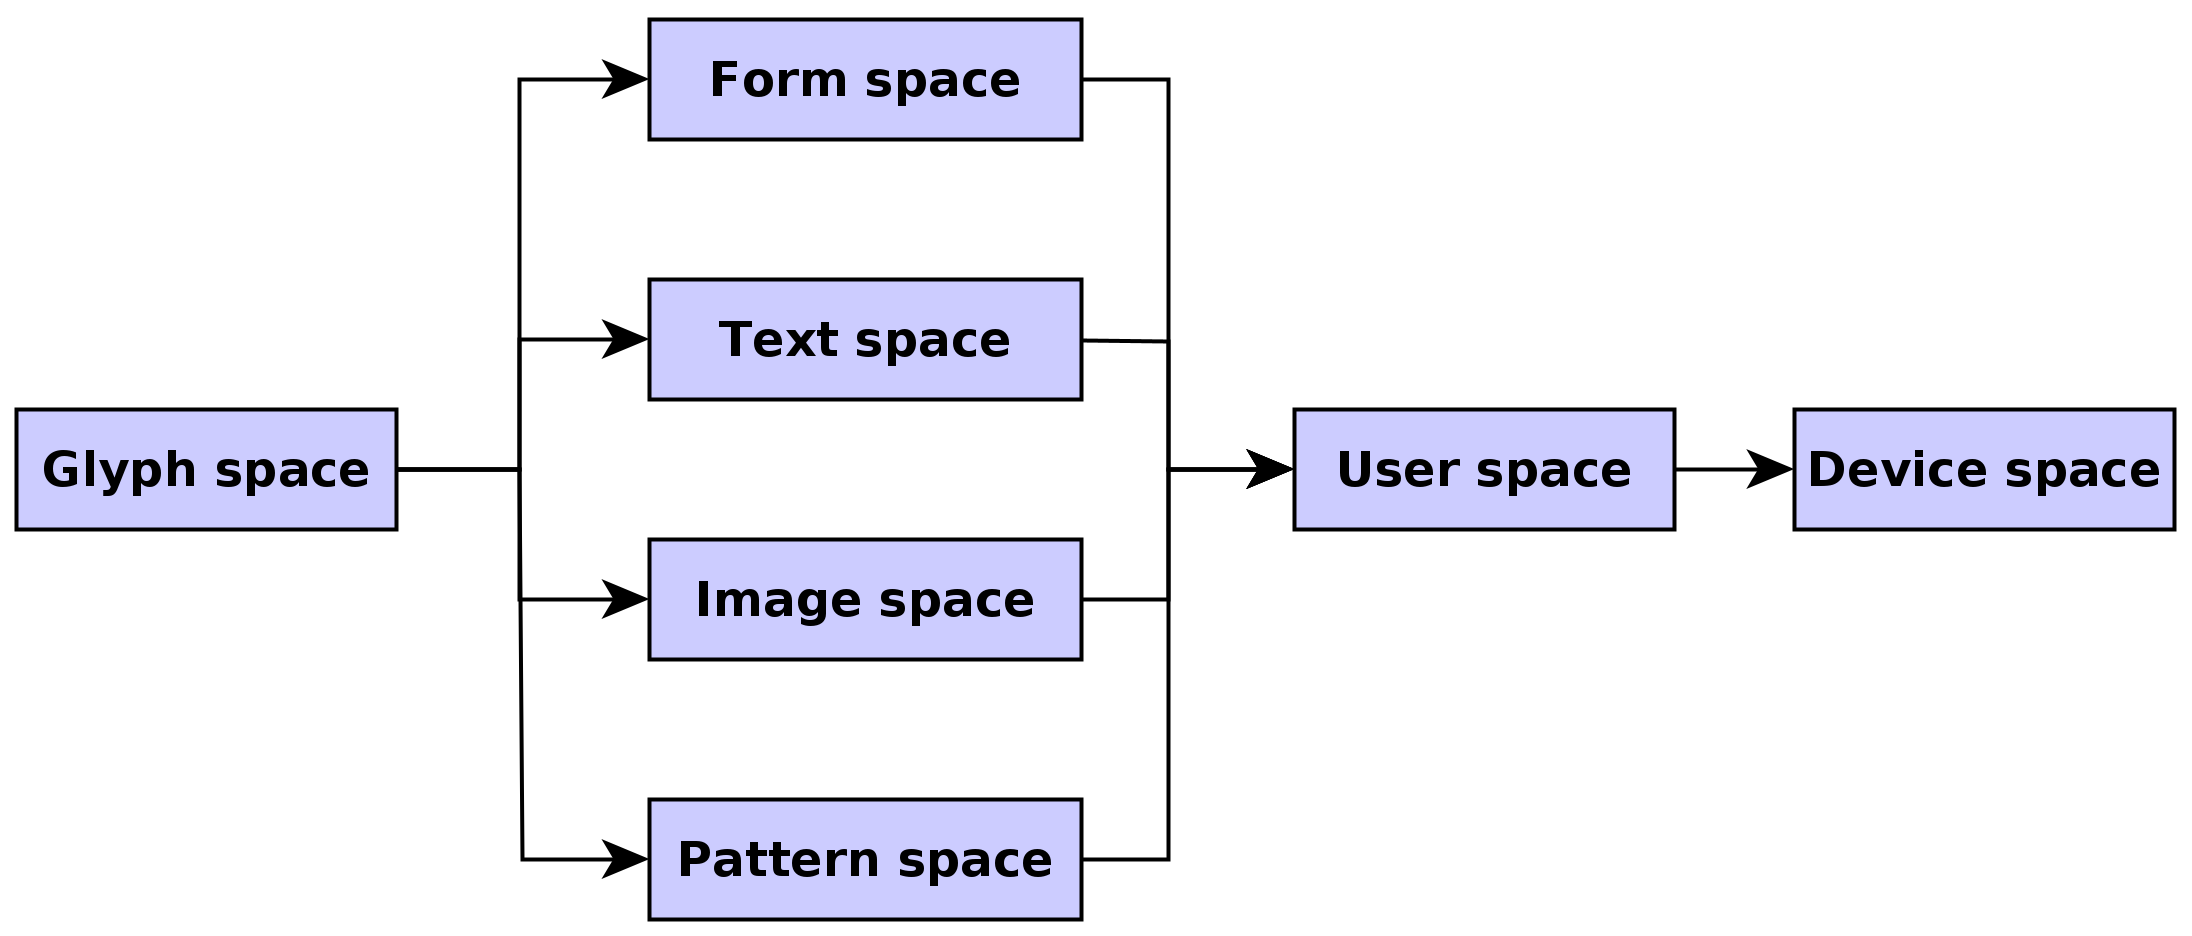
\includegraphics[width=11cm]{imaxes/espacios-coordenadas.png}
\end{figure}

¿Por qué el formato PDF almacena las coordenadas de las regiones?

\section{El formato HOCR}
\section{Herramientas y librerías}

\begin{itemize}
	\item Extracción de texto: Apache PDFBox, pdftotext
	\item OCR: Tesseract
	\item Pretty print de JSON: jq
\end{itemize}

%%%%             %%%%
%%%% METODOLOGÍA %%%%
%%%%             %%%%

\chapter{Metodología}
\label{chap:metodologia}

\section{Planificación económica}

La metodología utilizada para el desarrollo del proyecto es una metodología Scrum adaptada a las particularidades del proyecto. Una vez seleccionadas las herramientas de trabajo y llevada a cabo una primera versión del \emph{engine}, el desarrollo de cada modelo siguió un proceso iterativo. En términos de sprints serían los siguientes:

\lettrine{E}{l} comienzo de este proyecto consistió en una amplia búsqueda de aproximaciones y herramientas que orientasen la construcción del producto final.

También se hacía necesario decidir que tareas se considerarían como responsabilidad del software y cuales no. Se trataba de acotar el problema para obtener unos resultados satisfactorios. 

\section{Sprint a}

La primera de las tareas a abordar en el trabajo fue investigar la viabilidad del proyecto. Planteado el problema, no se conocía una solución directa. El resultado de esta primera fase de investigación fue conocer la existencia de los formatos para descripción del contenido del documentos digitalizados.

\begin{itemize}
    \item Investigación de qué herramientas utilizar en Linux para tratar con ficheros PDF.
    \item Información del formato HOCR
    \item Información sobre el formato PDF
    \item Uso de Tesseract
\end{itemize}

\section{Sprint b - Preparación del engine}
\begin{itemize}
    \item Estructura de directorios
    \item Creación del Makefile
    \item Creación de los scripts
    \begin{itemize}
        \item Generación único para cada petición
        \item Recepción de los ficheros
        \item Renombrado de los fichero para tratamiento seguro
        \item Discriminación de ficheros basados en texto y basados en imagen
        \item Extracción de texto con pdftotext
        \item Invocación de las aplicaciones para generar el lenguaje intermedio y el lenguaje estructurado
    \end{itemize}
\end{itemize}

\section{Primer modelo}
\section{Segundo modelo}
\section{Tercer modelo}
\section{Modelo n...}
\section{Sprint f - Adaptaciones para la interfaz gráfica}
\begin{itemize}
    \item \emph{Dockerizacion}
    \item Generación de imágenes para cada página de los PDF basados en texto
    \item Poblar el directorio de salida con los resultados
\end{itemize}

\section{Resultados de la planificación}

Aquí debe explicarse los desvíos en la planificación tanto temporales como económicos.

%%%%                       %%%%
%%%% ENTORNO DE DESARROLLO %%%%
%%%%                       %%%%

\chapter{Entorno de desarrollo}
\label{chap:entorno-desarrollo}

\lettrine{E}{l} entorno de desarrollo utilizado consistió en una distribución Ubuntu GNU/Linux con versiones actualizadas de las aplicaciones utilizadas en el proyecto. Para el desarrollo en lenguaje Python se optó por el IDE Eclipse con el plugin Pydev, específico para desarrollo con lenguaje Python. El codigo C y los scripts Bash fueron realizados con el editor Atom.

%%%%            %%%%
%%%% MATERIALES %%%%
%%%%            %%%%
\chapter{Materiales}
\label{chap:materiales}

Análisis de los documentos utilizados para el desarrollo del proyecto. Modelos PDF de texto facilitados por Betmedia. Modelos PDF imagen facilitados por Solco.

Caracterización de las regiones de interés.

Datos para identificar los documentos. En este caso, NIF, CIF.
